\section{Fórmulas}
\subsection{Física básica}
\subsubsection{Presión hidrostática $P_H$}
Es la presión ejercida por un líquido cuando no fluye.
\begin{figure}[h]
    \centering
    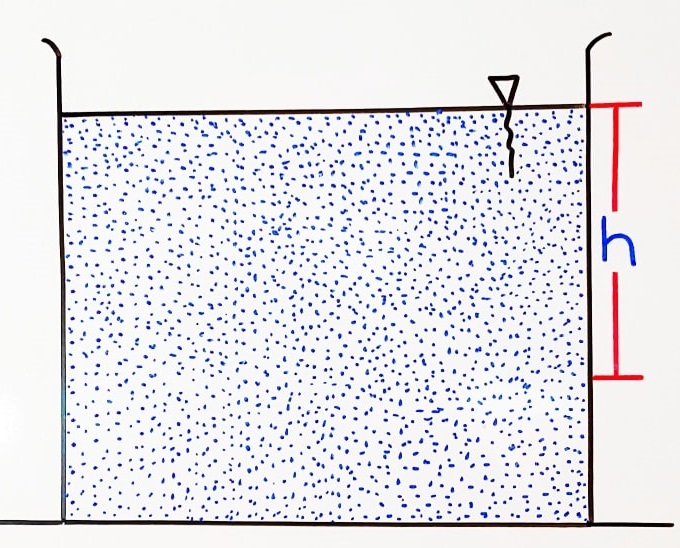
\includegraphics[width=4cm]{images/presión-hidrosta.jpg}
    %\caption{}
    \label{fig:{presion_hidrostatica}}
\end{figure}

La presión hidrostática está dado por:
$$P_H=\rho_{L} g h$$
Donde:\\
    $\rho_{L}$:densidad del líquido\\
    $g$: gravedad\\
    $h$: profundidad
